\section{When does Q choose the riskier signal?}\label{sec:16}

Straddles offer more dollar profit and much greater daily risk. At \(\lambda\) = 0.20, Q chooses put pairs alone on 141 later decision dates, straddles alone on 46, and an interior mix on four. It primarily switches strategies.


\begin{figure}[!htbp]\centering
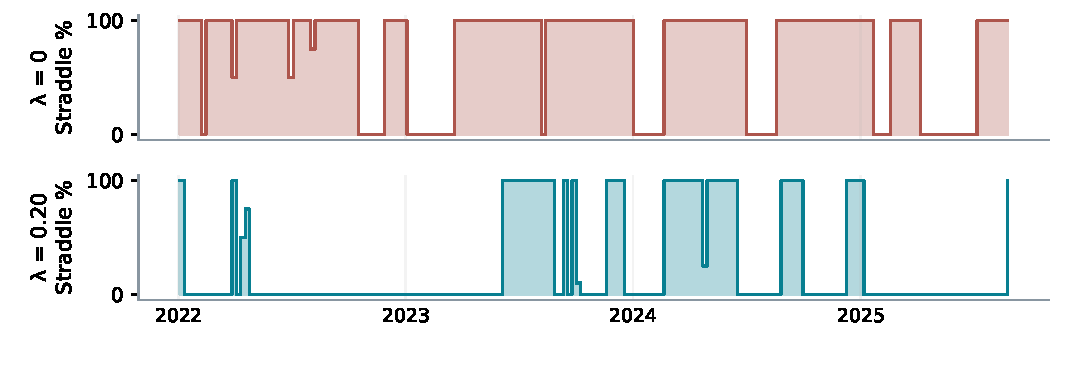
\includegraphics[width=\linewidth]{allocation_schedule.pdf}
\caption{Weekly target decisions during evaluation, before next-close execution. The remaining weight goes to put pairs. These are requested strategy allocations, not drifted portfolio holdings or individual trade sizes.}\label{fig:allocation-schedule}
\end{figure}

\subsection*{The selected intervals have different carry-to-risk ratios}

\begin{figure}[!htbp]\centering
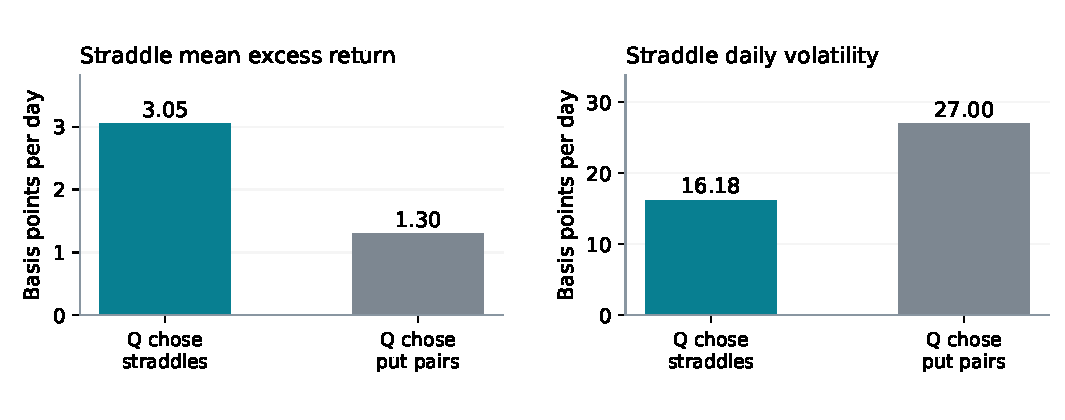
\includegraphics[width=\linewidth]{conditional_risk.pdf}
\caption{Realized straddle returns after \(\lambda\) = 0.20 Q decisions. Straddle-only choices cover 220 sessions; put-only choices cover 678. The four mixed-allocation intervals are omitted. Source costs are included; outer resizing charges are excluded.}\label{fig:conditional-risk}
\end{figure}

After Q chooses straddles, their mean daily excess return is 3.05 basis points with volatility 16.18; after it chooses put pairs, the straddle figures are 1.30 and 27.00. Put pairs average -0.09 basis points on the first set and +0.31 on the second. These are realized conditional statistics on noncontiguous dates, not causal estimates or standalone strategy Sharpes. Source costs are included; outer resizing charges are excluded.


A fixed target equal to Q's realized mean allocation reaches later Sharpe 1.387, versus 1.726 for Q: average exposure alone does not reproduce the result. The matched discount-zero learner reaches 1.645; continuation changes nine of 191 decisions at the same states. Much of the gain comes from conditional allocation, with a smaller incremental sequential benefit.


\FloatBarrier
